% ------------------------------------------------------------------------------------------------------------------------------------------
% ScaRC
% ------------------------------------------------------------------------------------------------------------------------------------------
\subsection{Scalable Recursive Clustering - \scarc{}} 
\label{SEC_SCARC_scarc}
  
With the aim to combine the advantages of the above Poisson solvers and to best possibly avoid their disadvantages the solution concept \scarc{} was developed. It can be understood as a combination of parallel Krylov and/or multigrid methods with techniques from multilevel domain decomposition to finally yield a robust, computationally and numerically efficient parallel solution for scalar elliptic equations. 

In fact, \scarc{} is not just a single solver, but rather a whole package of solvers and various components that can chosen in the view of the present situation. Its
design is focused on the following objectives: Most of the work required to solve the global problem should be done locally and coupled with as little communication effort as possible (high parallel efficiency). Convergence speed should be as high as possible and independent of the number of subdomains, the grid resolution and the complexity of the domain (high numerical efficiency). Further, the solver should be easily implementable and use only already existing standard methods. It should allow the application of optimized libraries and thus be able to make maximum use of the local processor power. Finally, it should guarantee the treatment of complicated geometries without lasting deterioration of the overall convergence rates. 

These are certainly very ambitious objectives that are extremely difficult to achieve at the same time. 
The following sections are concerned with describing the underlying algorithmic core concepts, their most important generalizations and a discussion on the performance achieved so far with regard to the above requirements.
%More detailed information can be found in \cite{Kilian2001, Kilian:1998, Goeddeke:2010, Wobker:2010}.


\subsubsection{Core algorithm}
\scarc{} is mainly defined as a symbiosis of global and local iterative techniques with the optional use of direct techniques locally. 
%As a fundamentally iterative method, \scarc{} is also based on defect correction techniques. 
The domain decomposition does not serve as a stand-alone solver, but rather to define suitable sub-problems that are only used to correct the globally defined solution.
%
In its original form \scarc{} only consists of the
nested combination of an outer (global) basic iteration and $M$ inner (local) basic iterations as displayed in Fig.~\ref{FIG_SCARC_basiciteration}. 

\begin{figure}[ht]
\begin{center}
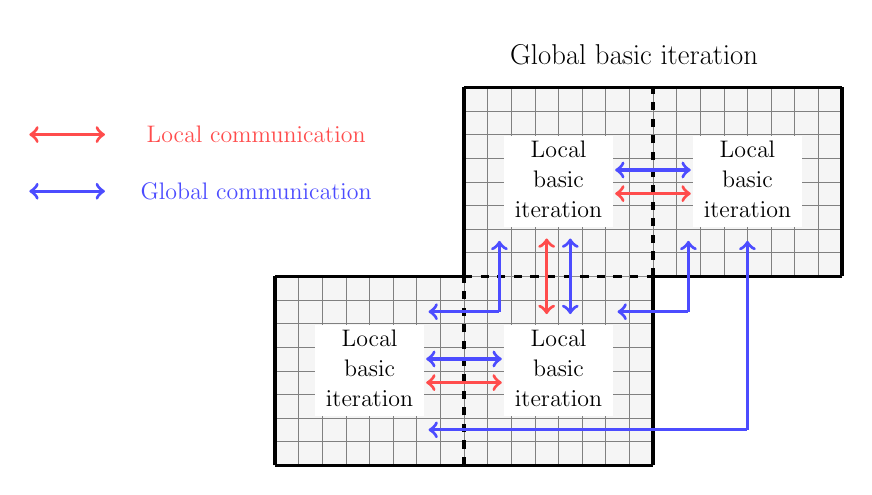
\begin{tikzpicture}
[
scale=0.6,
every node/.style={scale=0.6},
Background/.style={rectangle,draw=black!04,fill=black!04, thin, minimum size = 4 cm},
Obstruction/.style={rectangle,draw=black!70,fill=black!40, very thick, minimum size=1cm},
GlobalBorder/.style={-.,draw=black!100,  thin},
Finegrid/.style={step=0.5cm,gray,very thin},
Thickline/.style={-,draw=black!100,fill=black!02, very thick},
ThickDashedline/.style={-,draw=black!100,fill=black!02, very thick, dashed},
Thinline/.style={draw=black!100,fill=black!02, very thin},
Ball/.style={circle, draw=black!40, fill=red!20, thin, minimum size=3.5mm},
Circle/.style={circle,draw=black!40,fill=black!06,thin,minimum size=35.5mm},
Rectangle/.style={rectangle,draw=black!0,fill=white,inner xsep=0pt, inner ysep=0pt,},
Box/.style= {very thin, rectangle, inner xsep=10pt, inner ysep=10pt,},
ComRedArrow/.style= {very thick, draw=red!70,},
ComBlueArrow/.style= {very thick, draw=blue!70,},
DotArrow/.style= {<-, thick, dotted, draw=black!70,},
DotLine/.style= {very thick, dotted, draw=black!70,},
]

%\draw[GlobalBorder, fill=black!10] (-1.2,-1.2)--(13.2,-1.2)--(13.2,9.2)--(-1.2,9.2)--(-1.2,-1.2);
\node [Box, black] (box) at (7.6,8.7){\LARGE Global basic iteration};

\node[Background] at (  2,2) {};
\node[Background] at (  6,2) {};
\node[Background] at (  6,6) {};
\node[Background] at (10,6) {};

\node[Obstruction] at (2,2) {};

\draw[Finegrid] (0,0) grid (  8,4);
\draw[Finegrid] (4,4) grid (12,8);

\draw[Thickline] (0,0)--(  8,0);
\draw[Thickline] (4,8)--(12,8);
\draw[Thickline] (0,4)--(  4,4);
\draw[Thickline] (8,4)--(12,4);

\draw[Thickline] (  0,0)--(  0,4);
\draw[Thickline] (  4,8)--(12,8);
\draw[Thickline] (  4,4)--(  4,8);
\draw[Thickline] (  8,0)--(  8,4);
\draw[Thickline] (12,4)--(12,8);

\draw[ThickDashedline] (4,0)--(4,4);
\draw[ThickDashedline] (4,4)--(8,4);
\draw[ThickDashedline] (8,4)--(8,8);

\node[Rectangle] at (  2,2.0) {\Large \begin{tabular}{c} Local \\ basic \\iteration \end{tabular}};
\node[Rectangle] at (  6,2.0) {\Large \begin{tabular}{c} Local \\ basic \\iteration \end{tabular}};
\node[Rectangle] at (  6,6.0) {\Large \begin{tabular}{c} Local \\ basic \\iteration \end{tabular}};
\node[Rectangle] at (10,6.0) {\Large \begin{tabular}{c} Local \\ basic \\iteration \end{tabular}};

\draw[<->,ComRedArrow](3.2,1.75)--(4.8,1.75);
\draw[<->,ComRedArrow](5.75,3.2)--(5.75,4.8);
\draw[<->,ComRedArrow](7.2,5.75)--(8.8,5.75);

\draw[<->,ComBlueArrow](3.2,2.25)--(4.8,2.25);
\draw[<->,ComBlueArrow](6.25,3.2)--(6.25,4.8);
\draw[<->,ComBlueArrow](7.2,6.25)--(8.8,6.25);

\draw[<-, ComBlueArrow](3.25,3.25)--(4.75,3.25);
\draw[->, ComBlueArrow](4.75,3.25)--(4.75,4.75);
\draw[<-, ComBlueArrow](7.25,3.25)--(8.75,3.25);
\draw[->, ComBlueArrow](8.75,3.25)--(8.75,4.75);
\draw[<-, ComBlueArrow](3.25,0.75)--(10,0.75);
\draw[->, ComBlueArrow](10.0,0.75)--(10,4.75);
%

\draw[<->,ComRedArrow](-5.2,7.0)--(-3.6,7.0);
\node [Box,red!70] (box) at (-0.4,7.0){%
    \begin{minipage}{0.56\textwidth}
    \begin{center}
        {\Large Local communication}
    \end{center}
    \end{minipage}};
    
\draw[<->,ComBlueArrow](-5.2,5.8)--(-3.6,5.8);
\node [Box,blue!70] (box) at (-0.4,5.8){%
    \begin{minipage}{0.56\textwidth}
    \begin{center}
        {\Large Global communication}
    \end{center}
    \end{minipage}};

\end{tikzpicture}

\caption{Core component of \scarc{} consisting of a nested combination of a global basic iteration with local mesh-wise basic iterations.} 
\label{FIG_SCARC_basiciteration}
\end{center}
\end{figure}

\paragraph {\underline{Basic \scarc{} algorithm with domain decompositon preconditioner $B_S$} } \mbox{}\\[1ex]
Given an initial guess $x^0$, then solve the global system $Ax=b$ by the following steps:
\begin{enumerate}[(i)]
\item Perform a global basic iteration with a domain decomposition preconditioner $B_S$\,, 
\be 
x^k = x^{k-1} + B_S\, (b - Ax^{k-1})\,. 
\label{EQ_SCARC_global_basiciteration}
\ee
\item In each cycle $k$ of (i) simultaneously solve the related $M$ local systems for the restricted defects $d_i^{k-1}:= R_i\, {(b - A x^{k-1})}\,,$ 
\[ A_i y_i= d_i^{k-1}\,, \qquad i=1,\ldots, M\,,\] 
either by local direct solvers or by local basic iterations with preconditioners  $C_i=part(A_i)$  for the local Poisson matrices $A_i$ 
\be
y_i^{m} = y_i^{m-1} +  C_i \, ( d_i^{k-1} - A_i\, y_i^{m-1}   )\,, \qquad i=1,\ldots, M\,. 
\label{EQ_SCARC_local_basiciteration}
\ee  
\end{enumerate}
   
The outer basic iteration relies on a globally acting domain decomposition preconditioner $B_S$ for which various variants will be described below. 
The inner basic iterations are based on locally acting preconditioners $C_i$ which can be chosen individually for the different subdomains $\Omega_i$ depending on the local situation. Alternatively, the local problems can also be solved directly.

As will be explained in more detail below, this algorithmic core can be generalized in various ways. 
A formal description of the restriction operator $R_i$ which is used in part (ii) for the definition of the local defects can be found in Section (\ref{SEC_SCARC_block_precon}). Furthermore,
$C_i=part(A_i)$ means that only a partition of the local matrix $A_i$ is used for the preconditioning as e.g.\ its diagonal part $D_i$ which corresponds to a local Jacobi preconditioner. Again, different relaxation parameters $\omega_g$ and $\omega_l$  typically are used for the global and local iterations such that there actually holds
$B_S = B_S(\omega_g)$ and $C_i = C_i(\omega_l)$ which will be omitted for the sake of simplicity below.
%
A detailed description of the algorithmic concept and all related topics can be found in~\cite{Kilian:2001, Kilian:1998, Goeddeke:2010, Wobker:2010}.



\subsubsection{Multilevel Schwarz preconditioners}
For the preconditioning matrix $B_S$ %, for example, 
numerous variants with different degree of complexity can be applied.
All these variants have in common that they essentially rely on the solution of the local subdomain problems which are defined with respect to the original fine grid resolution. 
But they differ in the fact that, in addition to the fine grid level, an further coarse grid level can be used to ensure at least a basic transfer of global information. 
%
For the way in which the local sub-problems are coupled with each other and possibly with a coarse grid problem, there are again several possibilities. 
In addition, the local preconditioners $C_i$ can be chosen individually in best possible adjustment to the local conditions and
the accuracy requirements for the local solutions can be varied. 

To give a formal algorithmic description of the different variants, some notations related to the local fine grid preconditioners and the global coarse grid preconditioner are still introduced below.
In each cycle $k$ of the global basic iteration (\ref{EQ_SCARC_global_basiciteration}) 
the solution of the local basic iterations (\ref{EQ_SCARC_local_basiciteration}) makes use of the definitions below. 

First, the global defect, $d = b - Ax^{k-1}$, is restricted to the single subdomains, $d_i=R_i d$, then the corresponding local Poisson problems are solved, $v_i=A_i^{-1}d_i$, finally the local results are  prolonged back and summed up to a global solution, $v=\sum_{i=1}^M R_i^T v_i$. 
For each mesh the sequence of these steps can be summarized using the {\it local fine grid preconditioner} $B_i$ defined as follows
\[ B_i := R_i^T A_i^{-1}\,R_i\,,\qquad i=1,\ldots, M\,. \]

Second, if an additional coarse grid problem is used, then also a coarse Poisson matrix $A_C$ is required along with corresponding operators for prolongation, $R_C^T$, and restriction, $R_C$, 
which ensure the transfer between the fine and coarse level in a similar way.
Based on the same sequence of steps as for the $B_i$ above, the resulting {\it global coarse grid preconditioner} $b_C$ is then defined as
\[ b_C = R_C^T \,A_C^{-1}  R_C\,.\] 
Typically, the coarse grid consists of a finite difference discretization of the domain decomposition itself, i.e.\ $A_C \in {\bf R}^{M \times M}$, but it can also refer to a (still very) coarse refinement of it. 

The favored variants from the above-mentioned multitude of possibilities are presented and discussed below. 


% ------------------------  Additive 1-level Schwarz --------------------------------------------
\begin{enumerate}[(a)]
\item{{\bf Additive \ols{} (additive in fine level, no coarse level)}} \\[0.5ex]
The simplest variant for $B_S$ is based on the simultaneous solution of all local subdomain problems which is denoted as {\it additive} coupling. 
The {\it additive \ols{} preconditioner} $B_{AS1}$ is given by
\[B_{AS1} = \sum_{i=1}^M B_i \,. \]
Computationally, its application to a defect vector $B_{AS1}\,d\,$ is defined by 
\[  v \leftarrow \sum_{i=1}^M B_i\, d \,. \]

As the local calculations can be carried out completely in parallel
this type of preconditioning corresponds to a mesh-wise Jacobi scheme on subdomain level.

% ------------------------  Multiplicative 1-level Schwarz --------------------------------------------
\item{{\bf Multiplicative \ols{} (multiplicative in fine level, no coarse level)}} \\[0.5ex]
Alternatively, the subdomain problems can also be solved % in a staggered manner 
one after another which is denoted as {\it multiplicative} coupling. The  
{\it multiplicative \ols{} preconditioner} $B_{MS1}$ is formally given by
\[B_{MS1} = \left[ I - \prod_{i=1}^M (I - B_i\,A)\right] A^{-1}\,. \] 
Computationally, its application to a defect vector $B_{MS1}\,d\,$ is defined by 
\begin{eqnarray*}
v & \leftarrow & B_1\, d                               \,, \\
v & \leftarrow & v + B_j \, (d - Av)\,, \quad j=2 \ldots M\,. 
\end{eqnarray*}
Thus, new information obtained on mesh $j$ is passed to mesh $j+1$ as soon as it becomes available which may contribute to a clear improvement of the overall convergence speed.
This strategy basically corresponds to a Gauss-Seidel method on subdomain level, which, however, is immanently serial. So-called {\it red-black strategies} can be applied to increase the amount of parallelism, but this variant will be available only in the medium term. Thus, the coupling of the local sub-problems is always supposed to be of additive type for now.

% ------------------------  Additive 2-level Schwarz --------------------------------------------
\item{{\bf Additive \tls{} (additive in fine level, additive in coarse level)}}\\[0.5ex]
The two 1-level variants above are only based on the coupling of purely local solutions. But this strategy suffers from the same problem as the mesh-wise FFT: New information can only be distributed mesh-by-mesh throughout the entire domain, associated with a time delay which is proportional to the number of subdomains. 
By the additional use of a coarse grid problem, this dependency may be considerably mellowed and at least a rough assessment of the global information flow can be attained. 

If the coarse grid problem is additively coupled to the (also additive) local fine grid problems, then the {\it additive \tls{} preconditioner}  is given by
\[B_{AS2} = B_C + B_{AS1}  \,. \]
Computationally, its application to a defect vector $B_{AS2} \,d\,$ is defined by
\[  v \leftarrow  \left[B_C +  B_{AS1}\,\right] d \,. \]
The solution of the coarse grid problem and the fine grid problems is completely independent of each other leading to the highest possible parallel efficiency which can be achieved for 2-level methods. But both levels only use the last defect information of iteration $k-1$ such that new information is spread only in the following iteration once all solutions involved have been processed.

% ------------------------  Hybrid 2-level Schwarz --------------------------------------------
\item{{\bf Hybrid \tls{} (additive in fine level, multiplicative in coarse level)}}\\[0.5ex]
Alternatively, the computations of only one grid level can be carried out first, while those of the other level are performed afterwards which again corresponds to a multiplicative coupling. If the (additive) solution of the fine grid problems is completely done before the solution of the coarse grid problem, the resulting
{\it hybrid \tls{} preconditioner} $B_{HYB2}$ is given by
\[B_{HYB2} = B_C +  B_{AS1} - B_C \,A\, B_{AS1}\,. \] 
Computationally, its application to a defect vector $B_{HYB2}\, d$ is defined by 
\begin{eqnarray*}
v & \leftarrow & B_{AS1}\, d                            \,, \\
v & \leftarrow & v + B_C \, (d - Av)\,. 
\end{eqnarray*}
Now the latest available information from the fine grid problems can already be incorporated into a new defect calculation, which in turn is available for the next coarse grid problem. 
Despite the increased arithmetic and communication effort caused by the additional defect calculation, the associated gain in convergence speed is usually worth-while.

\end{enumerate}

The relation of additive to multiplicative Schwarz methods is similar to that of Jacobi and Gauss-Seidel methods.
It can be shown that the addition of a coarser grid level significantly reduces the dependence on the number of meshes.

\subsubsection{Algorithmic and performance-oriented aspects}
\label{SEC_SCARC_discussion}

\paragraph{Treatment of mesh interfaces:}
Since \scarc{} is based on a global discretization, there is no need to impose artificial boundary conditions along inner mesh boundaries or 
to use an additional pressure iteration to correct the velocity field there because internal boundary cells are treated as usual internal cells with respect to the virtual global matrix which is only handled in a distributed way. With a view to FDS, this has the advantage that the final global solution has consistent values along mesh interfaces by design, i.e.\ the normals of the single velocity components automatically match up to machine precision.

\paragraph{Accuracy of local solutions:}
Numerical experience has shown that block-wise schemes like the ones described before often perform well as long as complex parts 
are locally hidden and the local problems are solved with sufficient precision. In this light the quality of the local subdomain problems plays a major role. 
If the iterative processes are continued until machine precision for the local defect norms has been reached, the global basic iteration should be able to compute the same final solution as a corresponding direct solver that would be applied for the whole global problem.

However, in order to save computational costs, the iterative processes are typically stopped earlier, e.g.\ if only one digit or a moderately small tolerance has been reached or a fixed number of iterations has been performed.
According to the accuracy which is achieved locally at the end, the global basic iteration will in turn require more or less iterations to fulfil the globally desired stopping criterion. 

More accurate local solutions are certainly associated with an increase in arithmetic effort, but can also reduce the number of globally required iterations and thus the overall communication effort. Since {\it data processing} (the local computations) is still cheaper than {\it data movement} (the communications), this is usually worthwhile.
In this context, the local use of optimized libraries can make a significant contribution to an acceleration of the purely arithmetic components.
To sum up, the interplay between global and local effort must be balanced very well in order to achieve the shortest possible computing time and the highest possible convergence speed of the whole method.

\paragraph{Interplay of global and local iterations:}
The preconditioner $B_S$ is never built as a whole, but is rather available as a collection of local (and possibly global) components which are only implicitly represented by their action, i.e.\ solving the local sub-problems to a specified accuracy and exchanging shared data.
The single sub-problems are in turn only thought as corrections to a global solution vector, however, their parallel solution is much cheaper than that of a single global problem. By a suitable interaction of the different preconditioning components, the inevitable losses in global coupling (and thus numerical efficiency) induced by the domain decomposition can be significantly decreased.

A major advantage of the underlying methodology is that the local preconditioners can be defined completely independently of each other. The additive \ols{} preconditioner doesn't care how the local problems were solved, it just couples them together.
If particularly complex conditions exist in a certain subdomain, an optimized local multigrid method with a powerful recursive smoother could be used there, while in another subdomain only one SSOR-cycle might be enough to achieve the same local accuracy. This certainly leads to the fact that the arithmetic load on the individual subdomains can be very different depending on the local levels of difficulty such that a proper balance between numerical and computational efficiency must always be kept in mind.

\paragraph{Computational and communication effort:}
The overall communication effort of the different variants strongly depends on the choice of the global preconditioner $B_S$. As far as there is no coarse grid problem involved, 
the parallel efficiency is rather high because the preconditioning only needs local communication for the matrix-vector products in the defect computations. Apart from the coarse grid problem, which will be discussed immediately below, global communication is only needed for the computation of global defect norms to check the termination criterion of the global basic iteration.

The coarse grid solution can be achieved by any optimized direct solver which is typically performed on a selected `master' processor. This requires the communication of all related data between the subdomain processors to the master including synchronization overhead and possible waiting times (especially in case of unequal load distribution) which certainly leads to a considerable reduction of parallel efficiency.  
Alternatively, the coarse grid problem can be solved iteratively in a distributed fashion. However, this is associated with frequent exchanges of very small data associated with a correspondingly poor ratio of computational to communication overhead.

If the hybrid \tls{} preconditioner is used, the need to compute an additional defect (including next-neighbor communication) certainly increases the arithmetic costs per cycle of the \scarc{} basic iteration.
On the other hand, the 2-level variants are also associated with a considerable gain in numerical efficiency since information is used directly when it is available such that less global iterations are needed. Typically, the achieved acceleration of convergence speed makes up for the additional effort.

For decompositions with many subdomains, or in case that the coarse grid consists of a slightly refined version of the underlying domain decomposition, the coarse grid problem itself may be so large that it is no longer suitable for a direct solution. In this case the above 2-level concept can be applied recursively by solving the coarse grid problem again by a 2-level Schwarz method which leads to a full {\it multilevel Schwarz method}.


\paragraph{Adjusting algorithmic parameters:} 
A typical feature of iterative methods is that various parameters must be optimally adjusted which turns out to be a disadvantage of this concept. In particular, this applies to the global and local relaxation parameters which have a large influence on the convergence speed of the whole method up to divergence in the worst case. Their optimal choice depends on the problem characteristics and may be difficult to determine a-priori. However, appropriate sensitivity studies have already been capable of identifying related ranges which generally provide reasonable results.

\paragraph{Possible enhancements for multi-core architectures:}
If, as is possible in FDS, several meshes are mapped to one processor, the associated local mesh calculations are performed one after the other there. But instead of additively coupling these calculations as usual, a multiplicative coupling could now be considered within the scope of the processor, which might result in a further increase of the numerical efficiency in case of a clever clustering of the meshes. Furthermore, for the related meshes one common (unstructured) Poisson matrix could be assembled on the processor instead of the usual collection of locally structured matrices with corresponding overall solution of the locally clustered system. This strategy is only rudimentarily programmed so far and will be available in the medium term.



\subsubsection{Generalizations of the core algorithm}

As already discussed in section (\ref{SEC_SCARC_basic_iteration}) the convergence properties of the pure basic iteration are not satisfactory for complex situations. 
Thus, the efficiency of the global and local basic iterations can be significantly improved by incorporating Krylov and/or multigrid techniques on the global and/or the local layer as summarized in section (\ref{SEC_SCARC_generalizations}).

\paragraph{Generalizations of the global basic iteration:}
In the default version of \scarc{} currently available in FDS the outer basic iteration is simply replaced by a data-parallel global CG-method. 
Another powerful generalization is to use a data-parallel global MG-method with mesh-wise smoothing instead.
%
For the preconditioning/smoothing of both the global CG- and MG-methods  simply some steps of the local basic iterations can be performed, 
e.g.\ based on the SSOR-preconditioner leading to either a global CG-method with mesh-wise SSOR preconditioning or a global MG-method with mesh-wise SSOR smoothing.
%
As expected, the global CG-variants which only use a \ols{} preconditioner have a much better parallel efficiency than the global MG-variants because only a fine grid level with high computational complexity is used. But it should not be forgotten that the numerical efficiency of the CG-method may deteriorate significantly when the number of subdomains is increased 
which again is based on the lack of global data transfer for \ols{} preconditioners. The use of a suitable \tls{} preconditioner is able to remedy the situation, but associated with increased computational costs again.

In contrast, the global MG-variants show by far the better convergence behavior. This is mainly based on the stronger global coupling
which is achieved by the interlocking of levels with different resolutions and the addition of a coarse grid problem. 
Due to the restriction to local tensor product meshes, very sophisticated smoothers can be used which are capable of fully exploiting modern processor capabilities.
On the other hand, the coarse grid problem represents the already described bottleneck in terms of parallel efficiency. Furthermore, with every change to the next coarser grid level, the amount of local computational work decreases. Thus, during the changes to increasingly coarser grid levels, the related matrix vector products are associated with a decreasing ratio of local arithmetic work to communication work. These losses of parallel efficiency have to be taken into account when evaluating the overall efficiency and must clearly be compensated by the convergence acceleration induced by the use of different levels and the coarse grid solution.

A very special variant of \scarc{} is the combination of a global MG-method with optimized local MG-methods of Schwarz type. 
%In spite of the usual MG-features with a low degree of parallelizm, this double MG-structure leads to a very strong global coupling associated with a high numerical efficiency. 
Moreover, a further increase of efficiency may be achieved if the global MG-method is not used as standalone solver but in turn only as preconditioner inside a global CG-method, which provides an additional global coupling especially in case of big anisotropies on coarse grid level.
Again, the gain of numerical efficiency induced by these sophisticated combinations of different solution techniques must be set in relation to the associated increased effort.

\paragraph{Generalizations of the local basic iterations:}
There are numerous possibilities to also replace the local basic iterations with more efficient strategies. 
As those computations are performed completely locally, an obvious idea is to use the already described power of serial direct methods there. 
Thus, a favorite approach is to apply local FFT-methods or LU-decompositions. Alternatively, the local basic iterations can be replaced by local MG-methods with specially optimized local smoothers which are best possibly adapted to the underlying problem.


\paragraph{Important representatives and conclusion:}
In the light of the above discussions, the acronym \scarc{} can be explained now. It stands for:
\begin{itemize}
\item {\it Scalable}, with respect to the number of global (`k') and local solution steps (`m'),
\item {\it Recursive}, since it can be applied recursively to more than 2 levels with different refinements,
\item {\it Clustering}, since neighboring meshes can be merged into larger clusters with special treatment.
\end{itemize}

All in all, \scarc{} represents a large class of techniques, which contains a wide spectrum of the known Krylov, multigrid and domain decomposition approaches for the solution of discretized PDE's. 
The most important representatives are:
\vspace{-0.1cm}
\begin{enumerate}
\item set $k=1$ (globally), solve exactly (locally)      \\
  $\longrightarrow$ \, { Parallel CG-method with Additive \ols{} preconditioning}
\item set $m=1$ (locally) and $C_i=part(A_i)$ \\
  $\longrightarrow$ \, { Standard multigrid with mesh-wise smoothing}
\item set $m > 1$ (locally) and $C_i=part(A_i)$ and solve approximately (locally) via MG\\
  $\longrightarrow$ \,  { full \scarc{}}
\end{enumerate}
The first two variants are used in the course of the subsequent test calculations, see the definitions in Section \ref{SEC_SCARC_discretization_types}. 
The last variant is still under development, but will also be available shortly.

It becomes clear that \scarc{} is not a pure black-box solver and its application requires a careful assessment of the current circumstances. However, its major advantage is that it allows a very diverse combination of different components with regard to the selection of the global solvers (CG, MG or combinations of both), the local solvers (from simple Jacobi to highly optimized MG) and the local accuracy requirements (from gaining only one digit up to machine precision) such that any available information about the underlying problem can be exploited.



\subsubsection{Discretization types and application notes}
\label{SEC_SCARC_application_notes}

The \scarc{} functionality described in this documentation is not yet fully available in the latest precompiled FDS release.
To access the most recent version of \scarc{}, it is necessary to download a clone of the current FDS repository and compile the FDS code yourself. 
It must be emphasized that \scarc{} is still in a beta development state and there are still certain restrictions on its application. These actually still correspond to those for the \uglmat{} solver, namely that \scarc{} can only be applied for non-overlapping, non-stretched meshes at the same refinement level. While the use of an overlapping decomposition isn't necessary by design, the other two restrictions are only temporary in nature. Corresponding enhancements are basically possible and will be on the agenda in the immediate future.

In the recent past, many different cases from the verification and validation directory of FDS have been recalculated with \scarc{}.
Thereby, it has been proven repeatedly that the results obtained are algorithmically correct and that high accuracy can be achieved with completely correct transitions of the velocity field along inner mesh boundaries.
\newpage
However, particularly in case of longer lasting validation cases, it has also been observed that the previous runtimes are not yet optimal. This remaining weakness is mainly based on the fact that the focus of the development so far has been on the fundamental algorithmic correctness of the individual solution components. Nevertheless, there is still a great potential for runtime improvements and appropriate improvements will be done in the immediate future as well.

So far, there has been no discussion about what kind of discretization \scarc{} is working on. 
Basically, \scarc{} can be applied for structured and unstructured discretizations. Some application notes must be considered with respect to the globally and locally used components. Currently, the two following default versions for the structured and unstructured case are available:

\paragraph{Global structured discretization:}
The default variant for the structured case, simply abbreviated with \scarc{}, is illustrated in Figure \ref{FIG_default_scarc}. It can be called by setting {\ct SOLVER='SCARC'} in the {\ct \&PRES} name list and is based on a global, data-parallel CG method. The local Poisson matrices $A_i$ are assembled in a structured way, i.e.\ using the same matrix stencil everywhere and incorporating both gas-phase and solid cells.
Based on this structured type, the mesh-wise preconditioning is done by optimized local FFT from the CRAYFISHPAK package. 

Since there still may be velocity penetration errors towards internal obstructions, this variant is  embedded into the already known pressure iteration as explained in Section \ref{SEC_SCARC_fft_solver}. However, in contrast to the default FFT solver the velocity field is already correct along mesh interfaces and the pressure iteration only relates to internal obstructions.

\begin{figure}[ht]
\centering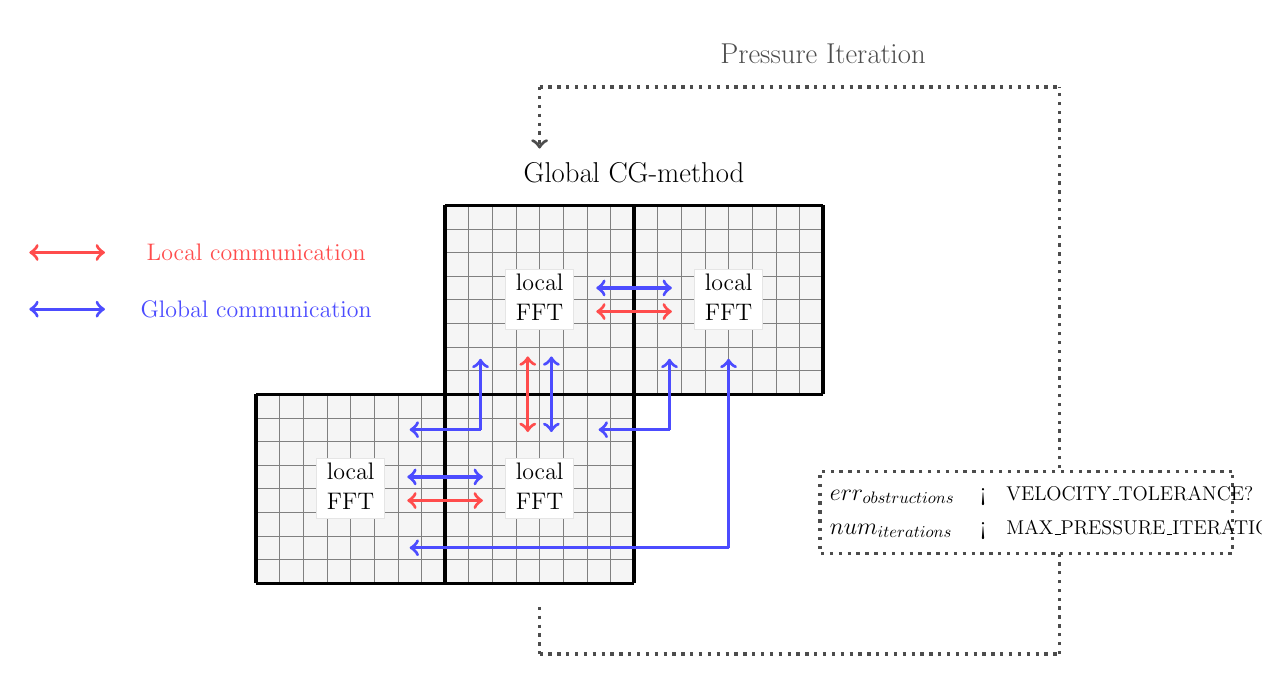
\begin{tikzpicture}
[
scale=0.6,
every node/.style={scale=0.6},
Background/.style={rectangle,draw=black!04,fill=black!04, thin, minimum size = 4 cm},
Obstruction/.style={rectangle,draw=black!70,fill=black!40, very thick, minimum size=1cm},
GlobalBorder/.style={-.,draw=black!100,  thin},
Finegrid/.style={step=0.5cm,gray,very thin},
Thickline/.style={-,draw=black!100,fill=black!02, very thick},
Thinline/.style={draw=black!100,fill=black!02, very thin},
Ball/.style={circle, draw=black!40, fill=red!20, thin, minimum size=3.5mm},
Circle/.style={circle,draw=black!40,fill=black!06,thin,minimum size=35.5mm},
Rectangle/.style={rectangle,draw=black!10,fill=white,inner xsep=0pt, inner ysep=0pt,},
Box/.style= {very thin, rectangle, inner xsep=10pt, inner ysep=10pt,},
DotBox/.style= {very thick, rectangle, inner xsep=0pt, inner ysep=8pt, dotted, fill=white, draw=black!70,},
ComRedArrow/.style= {very thick, draw=red!70,},
ComBlueArrow/.style= {very thick, draw=blue!70,},
DotArrow/.style= {<-, thick, dotted, draw=black!70,},
DotLine/.style= {very thick, dotted, draw=black!70,},
]

%\draw[GlobalBorder, fill=black!10] (-1.2,-1.2)--(13.2,-1.2)--(13.2,9.2)--(-1.2,9.2)--(-1.2,-1.2);
\node [Box, black] (box) at (8.0,8.7){\LARGE Global CG-method};

\node[Background] at (  2,2) {};
\node[Background] at (  6,2) {};
\node[Background] at (  6,6) {};
\node[Background] at (10,6) {};

\node[Obstruction] at (2,2) {};

\draw[Finegrid] (0,0) grid (  8,4);
\draw[Finegrid] (4,4) grid (12,8);

\draw[Thickline] (0,0)--(  8,0);
\draw[Thickline] (4,8)--(12,8);
\draw[Thickline] (0,4)--(  4,4);
\draw[Thickline] (8,4)--(12,4);

\draw[Thickline] (  0,0)--(  0,4);
\draw[Thickline] (  4,8)--(12,8);
\draw[Thickline] (  4,4)--(  4,8);
\draw[Thickline] (  8,0)--(  8,4);
\draw[Thickline] (12,4)--(12,8);

\draw[Thickline] (4,0)--(4,4);
\draw[Thickline] (4,4)--(8,4);
\draw[Thickline] (8,4)--(8,8);

\node[Rectangle] at (  2,2.0) {\Large \begin{tabular}{c} local \\ FFT\end{tabular}};
\node[Rectangle] at (  6,2.0) {\Large \begin{tabular}{c} local \\ FFT\end{tabular}};
\node[Rectangle] at (  6,6.0) {\Large \begin{tabular}{c} local \\ FFT\end{tabular}};
\node[Rectangle] at (10,6.0) {\Large \begin{tabular}{c} local \\ FFT\end{tabular}};

\draw[<->,ComRedArrow](3.2,1.75)--(4.8,1.75);
\draw[<->,ComRedArrow](5.75,3.2)--(5.75,4.8);
\draw[<->,ComRedArrow](7.2,5.75)--(8.8,5.75);

\draw[<->,ComBlueArrow](3.2,2.25)--(4.8,2.25);
\draw[<->,ComBlueArrow](6.25,3.2)--(6.25,4.8);
\draw[<->,ComBlueArrow](7.2,6.25)--(8.8,6.25);

\draw[<-, ComBlueArrow](3.25,3.25)--(4.75,3.25);
\draw[->, ComBlueArrow](4.75,3.25)--(4.75,4.75);
\draw[<-, ComBlueArrow](7.25,3.25)--(8.75,3.25);
\draw[->, ComBlueArrow](8.75,3.25)--(8.75,4.75);
\draw[<-, ComBlueArrow](3.25,0.75)--(10,0.75);
\draw[->, ComBlueArrow](10.0,0.75)--(10,4.75);

\draw[<->,ComRedArrow](-4.8,7.0)--(-3.2,7.0);
\node [Box,red!70] (box) at (-0.0,7.0){%
    \begin{minipage}{0.56\textwidth}
    \begin{center}
        {\Large Local communication}
    \end{center}
    \end{minipage}};
    
\draw[<->,ComBlueArrow](-4.8,5.8)--(-3.2,5.8);
\node [Box,blue!70] (box) at (-0.0,5.8){%
    \begin{minipage}{0.56\textwidth}
    \begin{center}
        {\Large Global communication}
    \end{center}
    \end{minipage}};
    
\draw[  -,DotLine](6,-0.5)--(6,-1.5);
\draw[  -,DotLine](6,-1.5)--(17,-1.5);
\draw[  -,DotLine](17,-1.5)--(17,10.5);
\draw[  -,DotLine](6,10.5)--(17,10.5);
\draw[->,DotLine](6,10.5)--(6,9.2);

\node [DotBox] (box) at (16.3,1.5){%
    \begin{minipage}{0.72\textwidth}    
    \begin{center}
    \begin{tabular}{lclc|c|}
       {\ct  \Large $err_{obstructions}$} & {\Large <} & {\ct \large VELOCITY\_TOLERANCE?}            \\[2ex]
       {\ct  \Large $num_{iterations}$ }    &{\Large <} & {\ct \large MAX\_PRESSURE\_ITERATIONS?} \\
    \end{tabular}
    \end{center}
    \end{minipage}};

\node [Box, black!70] (box) at (12,11.2){\LARGE Pressure Iteration};


\end{tikzpicture}

\caption{The default  \scarc{} version is defined on a global structured discretization, uses a global data-parallel CG-method with mesh-wise preconditioning by local optimized FFT-methods and is embedded in a pressure iteration to correct velocity penetration at internal obstructions.} 
\label{FIG_default_scarc}
\end{figure}

\newpage   %remove this if another page layout is requested
\paragraph{Global unstructured discretization:}
The default variant for the unstructured case, simply abbreviated with \uscarc{}, is illustrated in Figure 
\ref{FIG_default_uscarc}. It can be called by setting {\ct SOLVER='USCARC'} in the {\ct \&PRES} name list
and is also based on a global data-parallel CG method. The local Poisson matrices are assembled in an unstructured way, i.e.\  using individual matrix stencils and incorporating only gas-phase cells while setting no-flux boundary conditions along internal solids.
Based on this unstructured type, however, the 
mesh-wise preconditioning can no longer be done by local FFT's, but local $LU$-decompositions are used instead based on the {\tt PARDISO} solver of the Intel\textsuperscript{\textregistered} Math Kernel Library. Apart from the already correct transitions along inner mesh boundaries, the treatment of inner obstructions is also correct and no pressure iteration is needed anymore.

As the following test calculations will show, the local $LU$-decompositions are not as performant as the local FFT methods. For test cases whose structured execution by \scarc{} only requires a small number of pressure iterations, it can therefore happen that the corresponding more accurate \uscarc{} version, although it only requires one pressure iteration, is still slower. 
Strategies to improve this situation are currently being developed.

\begin{figure}[ht]
\centering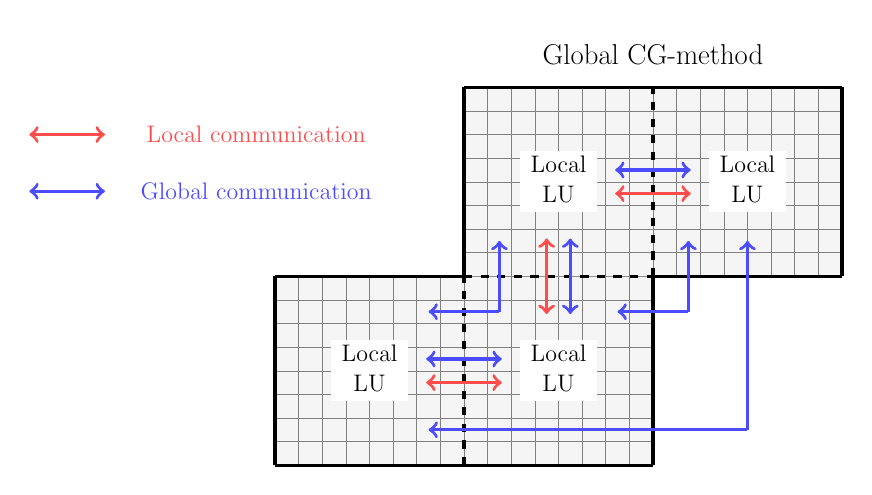
\begin{tikzpicture}
[
scale=0.6,
every node/.style={scale=0.6},
Background/.style={rectangle,draw=black!04,fill=black!04, thin, minimum size = 4 cm},
Obstruction/.style={rectangle,draw=black!70,fill=black!40, very thick, minimum size=1cm},
GlobalBorder/.style={-.,draw=black!100,  thin},
Finegrid/.style={step=0.5cm,gray,very thin},
Thickline/.style={-,draw=black!100,fill=black!02, very thick},
ThickDashedline/.style={-,draw=black!100,fill=black!02, very thick, dashed},
Thinline/.style={draw=black!100,fill=black!02, very thin},
Ball/.style={circle, draw=black!40, fill=red!20, thin, minimum size=3.5mm},
Circle/.style={circle,draw=black!40,fill=black!06,thin,minimum size=35.5mm},
Rectangle/.style={rectangle,draw=black!0,fill=white,inner xsep=0pt, inner ysep=0pt,},
Box/.style= {very thin, rectangle, inner xsep=10pt, inner ysep=10pt,},
DotBox/.style= {very thick, rectangle, inner xsep=10pt, inner ysep=10pt, dotted, fill=white, draw=black!70,},
ComRedArrow/.style= {very thick, draw=red!70,},
ComBlueArrow/.style= {very thick, draw=blue!70,},
DotArrow/.style= {<-, thick, dotted, draw=black!70,},
DotLine/.style= {very thick, dotted, draw=black!70,},
]

%\draw[GlobalBorder, fill=black!10] (-1.2,-1.2)--(13.2,-1.2)--(13.2,9.2)--(-1.2,9.2)--(-1.2,-1.2);
\node [Box, black] (box) at (8.0,8.7){\LARGE Global CG-method};

\node[Background] at (  2,2) {};
\node[Background] at (  6,2) {};
\node[Background] at (  6,6) {};
\node[Background] at (10,6) {};

\node[Obstruction] at (2,2) {};

\draw[Finegrid] (0,0) grid (  8,4);
\draw[Finegrid] (4,4) grid (12,8);

\draw[Thickline] (0,0)--(  8,0);
\draw[Thickline] (4,8)--(12,8);
\draw[Thickline] (0,4)--(  4,4);
\draw[Thickline] (8,4)--(12,4);

\draw[Thickline] (  0,0)--(  0,4);
\draw[Thickline] (  4,8)--(12,8);
\draw[Thickline] (  4,4)--(  4,8);
\draw[Thickline] (  8,0)--(  8,4);
\draw[Thickline] (12,4)--(12,8);

\draw[ThickDashedline] (4,0)--(4,4);
\draw[ThickDashedline] (4,4)--(8,4);
\draw[ThickDashedline] (8,4)--(8,8);

\node[Rectangle] at (  2,2.0) {\Large \begin{tabular}{c} Local \\ LU\end{tabular}};
\node[Rectangle] at (  6,2.0) {\Large \begin{tabular}{c} Local \\ LU\end{tabular}};
\node[Rectangle] at (  6,6.0) {\Large \begin{tabular}{c} Local \\ LU\end{tabular}};
\node[Rectangle] at (10,6.0) {\Large \begin{tabular}{c} Local \\ LU\end{tabular}};

\draw[<->,ComRedArrow](3.2,1.75)--(4.8,1.75);
\draw[<->,ComRedArrow](5.75,3.2)--(5.75,4.8);
\draw[<->,ComRedArrow](7.2,5.75)--(8.8,5.75);

\draw[<->,ComBlueArrow](3.2,2.25)--(4.8,2.25);
\draw[<->,ComBlueArrow](6.25,3.2)--(6.25,4.8);
\draw[<->,ComBlueArrow](7.2,6.25)--(8.8,6.25);

\draw[<-, ComBlueArrow](3.25,3.25)--(4.75,3.25);
\draw[->, ComBlueArrow](4.75,3.25)--(4.75,4.75);
\draw[<-, ComBlueArrow](7.25,3.25)--(8.75,3.25);
\draw[->, ComBlueArrow](8.75,3.25)--(8.75,4.75);
\draw[<-, ComBlueArrow](3.25,0.75)--(10,0.75);
\draw[->, ComBlueArrow](10.0,0.75)--(10,4.75);

\draw[<->,ComRedArrow](-5.2,7.0)--(-3.6,7.0);
\node [Box,red!70] (box) at (-0.4,7.0){%
    \begin{minipage}{0.56\textwidth}
    \begin{center}
        {\Large Local communication}
    \end{center}
    \end{minipage}};
    
\draw[<->,ComBlueArrow](-5.2,5.8)--(-3.6,5.8);
\node [Box,blue!70] (box) at (-0.4,5.8){%
    \begin{minipage}{0.56\textwidth}
    \begin{center}
        {\Large Global communication}
    \end{center}
    \end{minipage}};

\end{tikzpicture}

\caption{The default \uscarc{} version is defined on a global unstructured discretization and consists of a global data-parallel CG-method with mesh-wise preconditioning by local optimized LU-methods.} 
\label{FIG_default_uscarc}
\end{figure}
 
In general, MG methods must ensure that the number of grid cells in the various spatial dimensions can be divided by 2 at least once which may be an undesired restriction in geometric flexibility.
 The use of so-called {\it algebraic multigrid methods}, which work on arbitrary numbers of cells, is already well advanced, but will only be available in the medium term.
At the moment, the MG variant should only be used for structured discretizations (along with the already mentioned divisibility condition). In the unstructured case it may otherwise happen that during the coarsening process inner obstructions can no longer be resolved with the coarser grid width. 
An MG variant that basically uses structured grids on coarser levels, even if the fine grid level is unstructured, is in progress. Since the coarser levels only serve to correct the fine global problem, a combination of different discretization techniques is possible.
The same considerations currently holds true for the usage of the \tls{} preconditioners as they also require a divisibility of the grid size at least by 2.

\subsubsection{Description of parameters}

The following listing of \scarc{} related parameters in the {\ct \&PRES} namelist is still incomplete.
At this stage, it is not yet clear whether most of the \scarc{} parameters should remain hidden and only some basic parameters should be provided for user-defined variation. Once this is determined, a detailed explanation of the remaining parameters will follow.

\begin{longtable}{@{\extracolsep{\fill}}|l|l|l|l|l|}
\caption[SCARC parameters ({\ct PRES} name list group)]{For more information see Section (\ref{SEC_SCARC_cg}).}
\label{TBL_SCARC_parameters} \\
\hline
\multicolumn{5}{|c|}{{\ct PRES} (SCARC Parameters)} \\
\hline \hline
\endfirsthead
\caption[]{Continued} \\
\hline


\multicolumn{5}{|c|}{{\ct PRES} (SCARC Parameters)} \\
\hline \hline
\endhead
{\ct SCARC\_ACCURACY}                        & Character      & Section~\ref{SEC_SCARC_scarc}  & &  {\ct 'ABSOLUTE'}     \\ \hline
{\ct SCARC\_COARSE}                             & Character      & Section~\ref{SEC_SCARC_mg}  & &  {\ct 'ITERATIVE'}    \\ \hline
{\ct SCARC\_COARSE\_ACCURACY}      & Real              & Section~\ref{SEC_SCARC_mg}  & &  $10^{-14}$           \\ \hline
{\ct SCARC\_COARSE\_ITERATIONS}     & Integer          & Section~\ref{SEC_SCARC_mg}  & &  100                 \\ \hline
{\ct SCARC\_COARSE\_LEVEL}               & Integer          & Section~\ref{SEC_SCARC_mg}  & &  1                   \\ \hline
{\ct SCARC\_COARSE\_OMEGA}             & Real              & Section~\ref{SEC_SCARC_mg}  & &  0.8                 \\ \hline
{\ct SCARC\_CSV}                                     & Character      & Section~\ref{SEC_SCARC_scarc}  & &  {\ct 'NONE'}        \\ \hline
{\ct SCARC\_DEBUG}                               & Character      & Section~\ref{SEC_SCARC_scarc}  & &  {\ct 'NONE'}        \\ \hline
{\ct SCARC\_DISCRETIZATION}              & Character      & Section~\ref{SEC_SCARC_poisson}  & &  {\ct 'STRUCTURED'}  \\ \hline
{\ct SCARC\_KRYLOV}                             & Character      & Section~\ref{SEC_SCARC_cg}  & &  {\ct 'CG'}          \\ \hline
{\ct SCARC\_KRYLOV\_ACCURACY}      & Character      & Section~\ref{SEC_SCARC_cg}  & &  $10^{-10}$          \\ \hline
{\ct SCARC\_KRYLOV\_INTERPOL}        & Character      & Section~\ref{SEC_SCARC_cg}  & &  {\ct 'CONSTANT'}    \\ \hline
{\ct SCARC\_KRYLOV\_ITERATIONS}     & Integer           & Section~\ref{SEC_SCARC_cg}  & &  500                 \\ \hline
{\ct SCARC\_METHOD}                             & Character      & Section~\ref{SEC_SCARC_scarc}  & &  {\ct 'NONE'}        \\ \hline
{\ct SCARC\_MULTIGRID}                         & Character      & Section~\ref{SEC_SCARC_mg}  & &  {\ct 'GEOMETRIC'}   \\ \hline
{\ct SCARC\_MULTIGRID\_ACCURACY}   & Real             & Section~\ref{SEC_SCARC_mg}  & &  $10^{-10}$          \\ \hline
{\ct SCARC\_MULTIGRID\_COARSENING} & Character   & Section~\ref{SEC_SCARC_mg}  & &  {\ct 'FALGOUT'}     \\ \hline
{\ct SCARC\_MULTIGRID\_CYCLE}            & Character     & Section~\ref{SEC_SCARC_mg}  & &  {\ct 'V'}           \\ \hline
{\ct SCARC\_MULTIGRID\_INTERPOL}      & Character     & Section~\ref{SEC_SCARC_mg}  & &  {\ct 'CONSTANT'}    \\ \hline
{\ct SCARC\_MULTIGRID\_ITERATIONS}   & Integer         & Section~\ref{SEC_SCARC_mg}  & &  100                 \\ \hline
{\ct SCARC\_MULTIGRID\_LEVEL}             & Integer         & Section~\ref{SEC_SCARC_scarc}  & &  -1                  \\ \hline
{\ct SCARC\_PRECISION}                          & Character      & Section~\ref{SEC_SCARC_cg}  & &  {\ct 'DOUBLE'}      \\ \hline
{\ct SCARC\_PRECON}                              & Character      & Section~\ref{SEC_SCARC_cg}  & &  {\ct 'NONE'}        \\ \hline
{\ct SCARC\_PRECON\_ACCURACY}      & Real              & Section~\ref{SEC_SCARC_cg}  & &  $10^{-10}$          \\ \hline
{\ct SCARC\_PRECON\_ITERATIONS}     & Integer           & Section~\ref{SEC_SCARC_cg}  & &  100                 \\ \hline
{\ct SCARC\_PRECON\_OMEGA}            & Real              & Section~\ref{SEC_SCARC_mg}  & &  0.8                 \\ \hline
{\ct SCARC\_SMOOTH}                            & Character       & Section~\ref{SEC_SCARC_mg}  & &  {\ct 'SSOR'}        \\ \hline
{\ct SCARC\_SMOOTH\_ACCURACY}      & Real              & Section~\ref{SEC_SCARC_mg}  & &  $10^{-8}$           \\ \hline
{\ct SCARC\_SMOOTH\_ITERATIONS}    & Integer           & Section~\ref{SEC_SCARC_mg}  & &  5                   \\ \hline
{\ct SCARC\_SMOOTH\_OMEGA}           & Real               & Section~\ref{SEC_SCARC_mg}  & &  0.8                 \\ \hline
{\ct SCARC\_TWOLEVEL}                        & Character         & Section~\ref{SEC_SCARC_scarc}  & &  {\ct 'STRUCTURED'}  \\ \hline
{\ct SCARC\_VERBOSE}                          & Character         & Section~\ref{SEC_SCARC_scarc}  & &  {\ct 'NONE'}        \\ \hline

\end{longtable}

